\documentclass[tikz,border=10pt]{standalone}
% Shared preamble for the CenterTask panel files (panel_a/b/c.tex).
% Edit colours and node styles here, once.
\usepackage{amsmath}
\usetikzlibrary{arrows.meta,positioning,calc}

% category colours as in ColorCategoryMap.m: 1=Short/Orange, 2=Mid/Green, 3=Long/Blue
\definecolor{catShort}{RGB}{243,178,132}
\definecolor{catMid}{RGB}{158,209,172}
\definecolor{catLong}{RGB}{157,188,234}

\tikzset{ctpanel/.style={
  font=\sffamily,
  band/.style={rounded corners=6pt, fill=black!7, draw=none, inner sep=8pt, minimum height=1.15cm},
  unit/.style={circle, fill=catMid!60, draw=none, minimum size=0.95cm, inner sep=0pt},
  flow/.style={-{Latex[length=2.2mm]}, line width=0.8pt},
  rowlab/.style={anchor=east, font=\sffamily\large},
  now/.style={fill=catShort!55, rounded corners=3pt, inner sep=3pt},
  stage/.style={rounded corners=6pt, fill=black!8, draw=none, inner sep=8pt, minimum height=1.2cm, align=center},
  target/.style={circle, minimum size=0.9cm, inner sep=0pt, draw=none, font=\sffamily\scriptsize, text=black!75},
  axis/.style={line width=0.6pt},
}}


\begin{document}
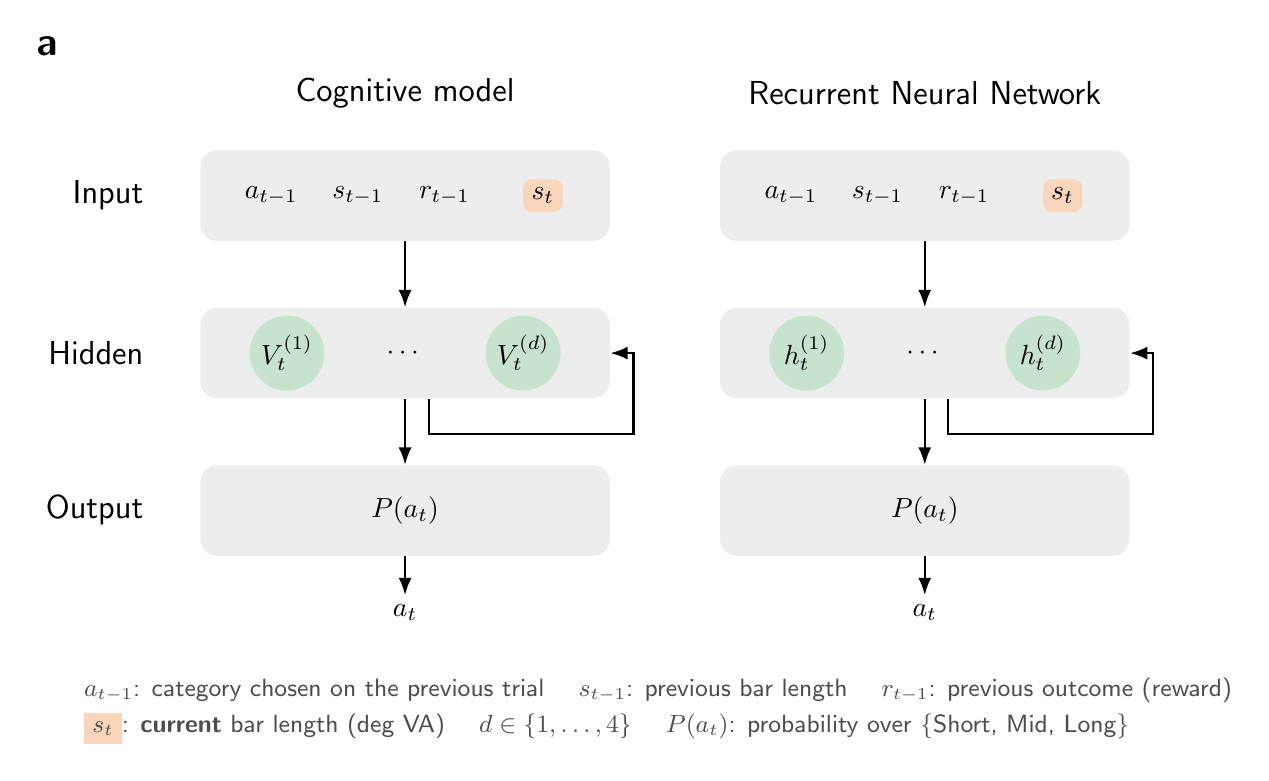
\begin{tikzpicture}[ctpanel]
% =====================================================================
%  (a)  Trial-level model: cognitive model vs recurrent neural network, with s_t added
% =====================================================================
\node[font=\sffamily\bfseries\Large, anchor=west] at (-2.2,1.9) {a};

\node[rowlab] at (-0.6, 0)   {Input};
\node[rowlab] at (-0.6,-2.0) {Hidden};
\node[rowlab] at (-0.6,-4.0) {Output};

\begin{scope}[xshift=0cm]
  \node[font=\sffamily\large] at (2.6, 1.3) {Cognitive model};
  \node[band, minimum width=5.2cm] (Lin) at (2.6,0) {};
  \node at (0.9,0) {$a_{t-1}$};
  \node at (2.0,0) {$s_{t-1}$};
  \node at (3.1,0) {$r_{t-1}$};
  \node[now] at (4.35,0) {$s_{t}$};
  \node[band, minimum width=5.2cm] (Lh) at (2.6,-2.0) {};
  \node[unit] at (1.1,-2.0) {$V_t^{(1)}$};
  \node at (2.6,-2.0) {$\cdots$};
  \node[unit] at (4.1,-2.0) {$V_t^{(d)}$};
  \node[band, minimum width=5.2cm] (Lout) at (2.6,-4.0) {$P(a_t)$};
  \node (La) at (2.6,-5.3) {$a_t$};
  \draw[flow] (Lin.south) -- (Lh.north);
  \draw[flow] (Lh.south) -- (Lout.north);
  \draw[flow] (Lout.south) -- (La);
  \draw[flow] (Lh.south) ++(0.3,0) |- ++(2.6,-0.45) |- (Lh.east);
\end{scope}

\begin{scope}[xshift=6.6cm]
  \node[font=\sffamily\large] at (2.6, 1.3) {Recurrent Neural Network};
  \node[band, minimum width=5.2cm] (Rin) at (2.6,0) {};
  \node at (0.9,0) {$a_{t-1}$};
  \node at (2.0,0) {$s_{t-1}$};
  \node at (3.1,0) {$r_{t-1}$};
  \node[now] at (4.35,0) {$s_{t}$};
  \node[band, minimum width=5.2cm] (Rh) at (2.6,-2.0) {};
  \node[unit] at (1.1,-2.0) {$h_t^{(1)}$};
  \node at (2.6,-2.0) {$\cdots$};
  \node[unit] at (4.1,-2.0) {$h_t^{(d)}$};
  \node[band, minimum width=5.2cm] (Rout) at (2.6,-4.0) {$P(a_t)$};
  \node (Ra) at (2.6,-5.3) {$a_t$};
  \draw[flow] (Rin.south) -- (Rh.north);
  \draw[flow] (Rh.south) -- (Rout.north);
  \draw[flow] (Rout.south) -- (Ra);
  \draw[flow] (Rh.south) ++(0.3,0) |- ++(2.6,-0.45) |- (Rh.east);
\end{scope}

\node[align=left, anchor=north west, font=\sffamily\small, text=black!70] at (-1.6,-6.0) {%
  $a_{t-1}$: category chosen on the previous trial \quad
  $s_{t-1}$: previous bar length \quad
  $r_{t-1}$: previous outcome (reward)\\[2pt]
  \colorbox{catShort!55}{$s_t$}: \textbf{current} bar length (deg VA) \quad
  $d \in \{1,\dots,4\}$ \quad
  $P(a_t)$: probability over \{Short, Mid, Long\}
};
\end{tikzpicture}
\end{document}
